Nakon što su obrasci skenirani, obrađeni, slova segmentirana i pripremljena za daljnju obradu na red dolazi određivanje razreda, odnosno slova abecede, pojedinoj slici slova, to jest klasifikacija. Za klasifikaciju prikupljenoga skupa podataka korištena je slojevita potpuno povezana unaprijedna umjetna neuronska mreža koja je učena algoritmom propagacije pogreške unatrag, točnije jednom varijantom navedenoga algoritma koja koristi inerciju kako bi se pospješilo i ubrzalo učenje.

\section{Motivacija i povijesni razvoj}

U današnje doba, uz nevjerojatne brojke o količini memorije, brzine procesora i razno raznih tehničkih detalja koji se iznose prilikom predstavljanja super-računala te o količini podataka koje obrađuju, ta brojka još uvijek nije ni blizu onoj brojci podataka koja se u svakom trenutku obrađuju u mozgu i živčanom sustavu živih bića. Ponukani tom idejom, Warren McCulloch i Walter Pitts u svom su radu \emph{A logical calculus of the ideas immanent in nervous activity} još 40-ih godina prošlog stoljeća predstavili model umjetnog neurona \engl{TLU perceptron} i pokazali da se njime mogu računati logičke funkcije I, ILI i NE, iz čega slijedi da se kombinacijom više tih neurona u neuronsku mrežu može dobiti proizvoljno kompleksna Booleova funkcija \citep{nenr}.

Nekoliko godina nakon navedenoga dvojca, britanski biolog Donald Hebb je u svojoj knjizi \emph{The Organization of Behavior} izjavio da \emph{učiti znači mijenjati jakosti veza između neurona}, što je Frank Rosenblatt 1957. godine iskoristio kao temelj za ostvarivanje algoritma učenja TLU perceptrona, što je bio velik uspjeh jer je uspio pokazati da se određeni problemi mogu rješavati učenjem, a ne samo konstrukcijom, kako su to Pitts i McCulloch pokazali.

Sam razvoj neuronskih mreža počeo je kao pokušaj da se objasni inteligentno ponašanje ljudi i životinja i to putem simbolističkog pristupa koji je kao cilj imao znanje iz neke domene obuhvatiti skupom atomičkih semantičkih objekata (simbola) i zatim činit niz manipulacija tih simbola pomoću algoritamskih pravila, no daljnjim istraživanjem mozga pokazano je da je takav pristup neutemeljen i nemoguć prilikom oponašanja inteligentnih bića jer su mozak i živčani sustav sastavljeni od velikog broja procesnih elemenata, odnosno neurona, koji obrađuju velike količine informacija paralelno, što je temelj pristupa koji je danas poznat pod nazivom konektivizam.

\section{Osnovni model umjetnog neurona}
Neuron, kao osnovna građevna jedinica živčanog sustava, prikazan je na slici \ref{fig:biological_neuron}. Ukratko, svaki neuron čini \emph{tijelo stanice} koje sadrži jezgru. Na rubovima tijela stanice nalaze se \emph{dendirit}, koji služe kao poveznica s ostalim neuronima te dovode impuls do \emph{tijela stanice}. Iz neurona kao izlaz prema ostalim neuronima služi produžetak nazvan \emph{akson}. U tijelu stanice vlada određeni električni potencijal, te promjenom tog potencijala nastaje elektrokemijski impuls koji se dalje širi aksonom koji je povezan s dendritima do 10000 drugih neurona. Prijenosom impulsa od neurona do neurona zapravo se odvija proces prijenos informacija koji je određen jakostima sinaptičkih veza između pojedinih neurona.
\begin{figure}[htb]
    \centering
    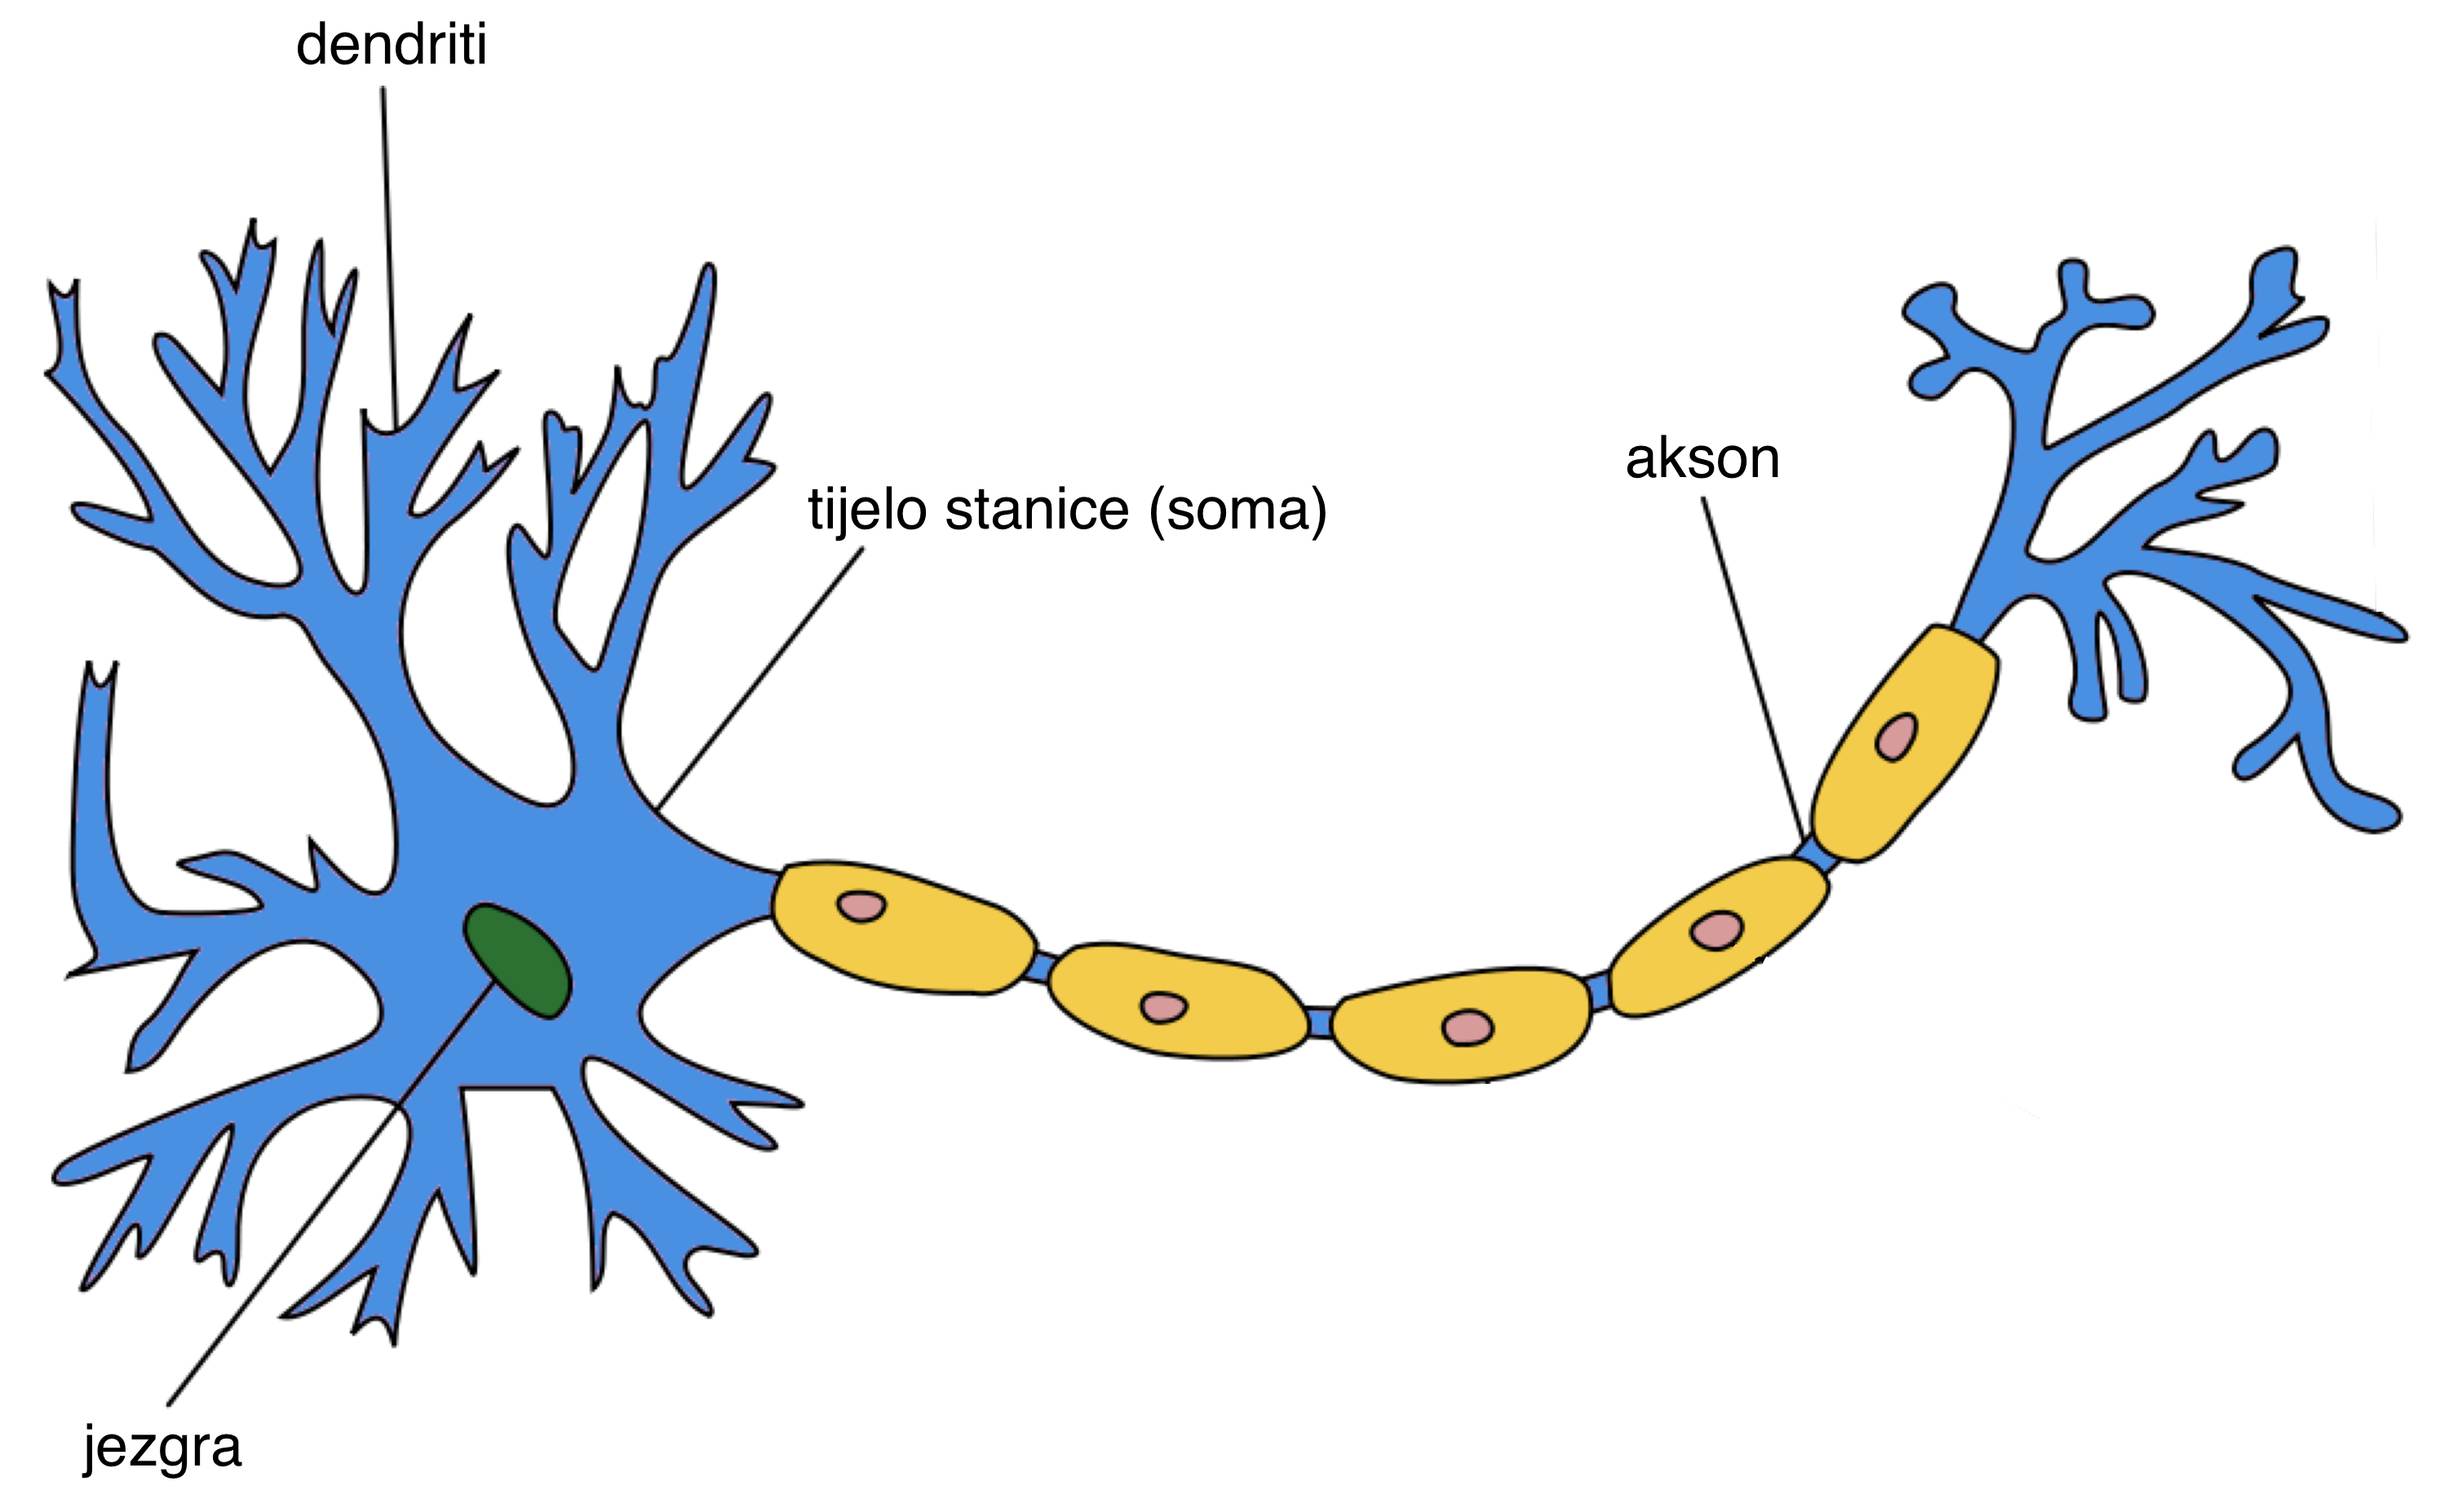
\includegraphics[width=14cm]{images/biological_neuron.jpg}
    \caption{Biološki neuron, preuzeto iz \citep{wikiNeuron}}
    \label{fig:biological_neuron}
\end{figure}

Kako je već spomenuto Warren McCulloch i Walter Pitts su 1943. godine povukli analogiju s biološkim neuronom te definirali model umjetnog neurona prikazanog na slici \ref{fig:neuron_model}. Umjetni model neurona se sastoji od ulaza $x_1, x_2, ..., x_n$ koji predstavljaju dendrite, preko kojih neuron prima pobudu od drugih neurona ili vanjskog svijeta. Utjecaj pojedinog ulaza na neuron definiran je težinama $w_1, w_2, ..., w_n$. Djelovanje pojedinog ulaza, to jest u kojoj mjeri pobuđuje neuron, definirano je umnoškom $w_1 \cdot x_1$.
\begin{figure}[htb]
    \centering
    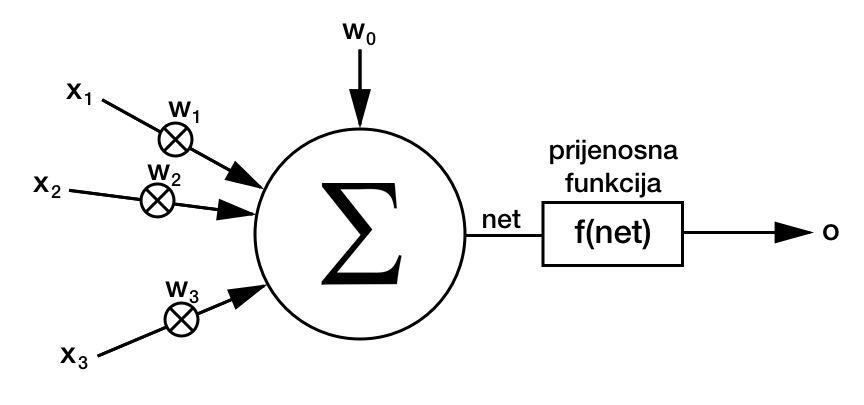
\includegraphics[width=14cm]{images/neuron_model.png}
    \caption{Osnovni model umjetnog neuron}
    \label{fig:neuron_model}
\end{figure}
Tijelo neurona se ponaša kao zbrajalo te na svom izlazu \emph{net} daje ukupnu pobudu. Ukupna pobuda neurona definirana je izrazom: $$net = \sum_{i=0}^{n} w_i \cdot x_i$$ gdje $x_0$ predstavlja fiktivni ulaz čija je vrijednost uvijek 1 (tako je prikazano radi ljepšeg zapisa), te težina $w_0$ predstavlja prag paljenja neurona.

Prijenosna funkcija \engl{transfer function} modelira ponašanje aksona te određuje konačni izlaz neurona u ovisnosti o ukupnoj pobudi. Prilikom modeliranja TLU perceptrona, McCulloch i Pitts su koristili prijenosnu funkciju skoka prikazanu na slici \ref{fig:step} te definiranu izrazom:
\[
  f(net) = \left\{\def\arraystretch{1.2}%
  \begin{array}{@{}c@{\quad}l@{}}
    0, & \text{$net \leq 0$} \\
    1, & \text{inače.}\\
  \end{array}\right.
\]
Bitno je napomenuti da se od neurona koji koriste linearne prijenosne funkcije ne mogu graditi složene neuronske mreže, jer se od linearnih elemenata ne može dobiti ništa složenije, to jest cijela se mreža opet pretvara u linearni element.
\begin{figure}[htb]
    \centering
    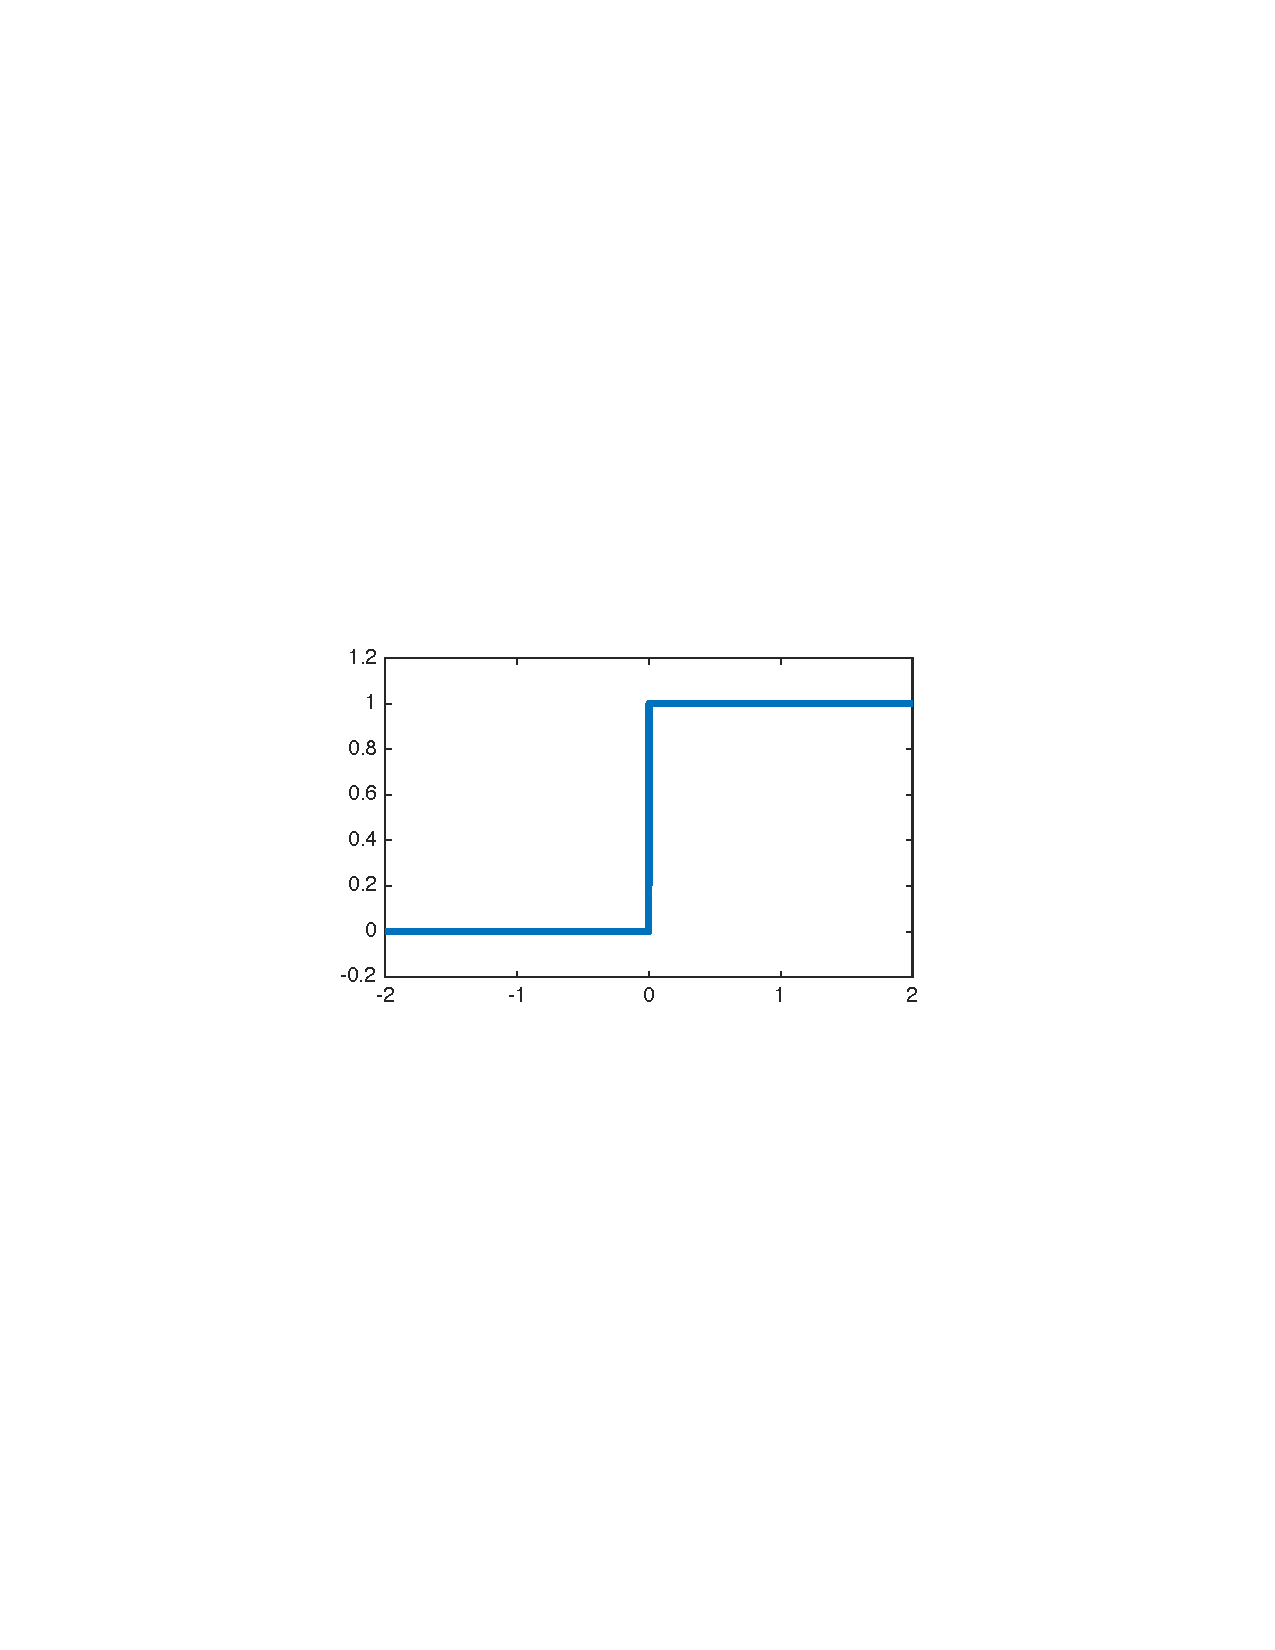
\includegraphics[width=10cm]{images/step.pdf}
    \caption{Funkcija skoka}
    \label{fig:step}
\end{figure}

U početku je bio velik problem definiranje algoritma učenja složenijih neuronskih mreža. No riješenje navedenoga problema se pojavilo u obliku algoritma propagacije pogreške unatrag uvođenjem derivabilnih prijenosnih funkcija. Najpoznatiji predstavnik te skupine prijenosnih funkcija je sigmoidalna (logistička) funkcija prikazana na slici \ref{fig:sigmoidal}, te definirana sljedećim izrazom: $$f(net) = \frac{1}{1+e^{-net}}$$
\begin{figure}[htb]
    \centering
    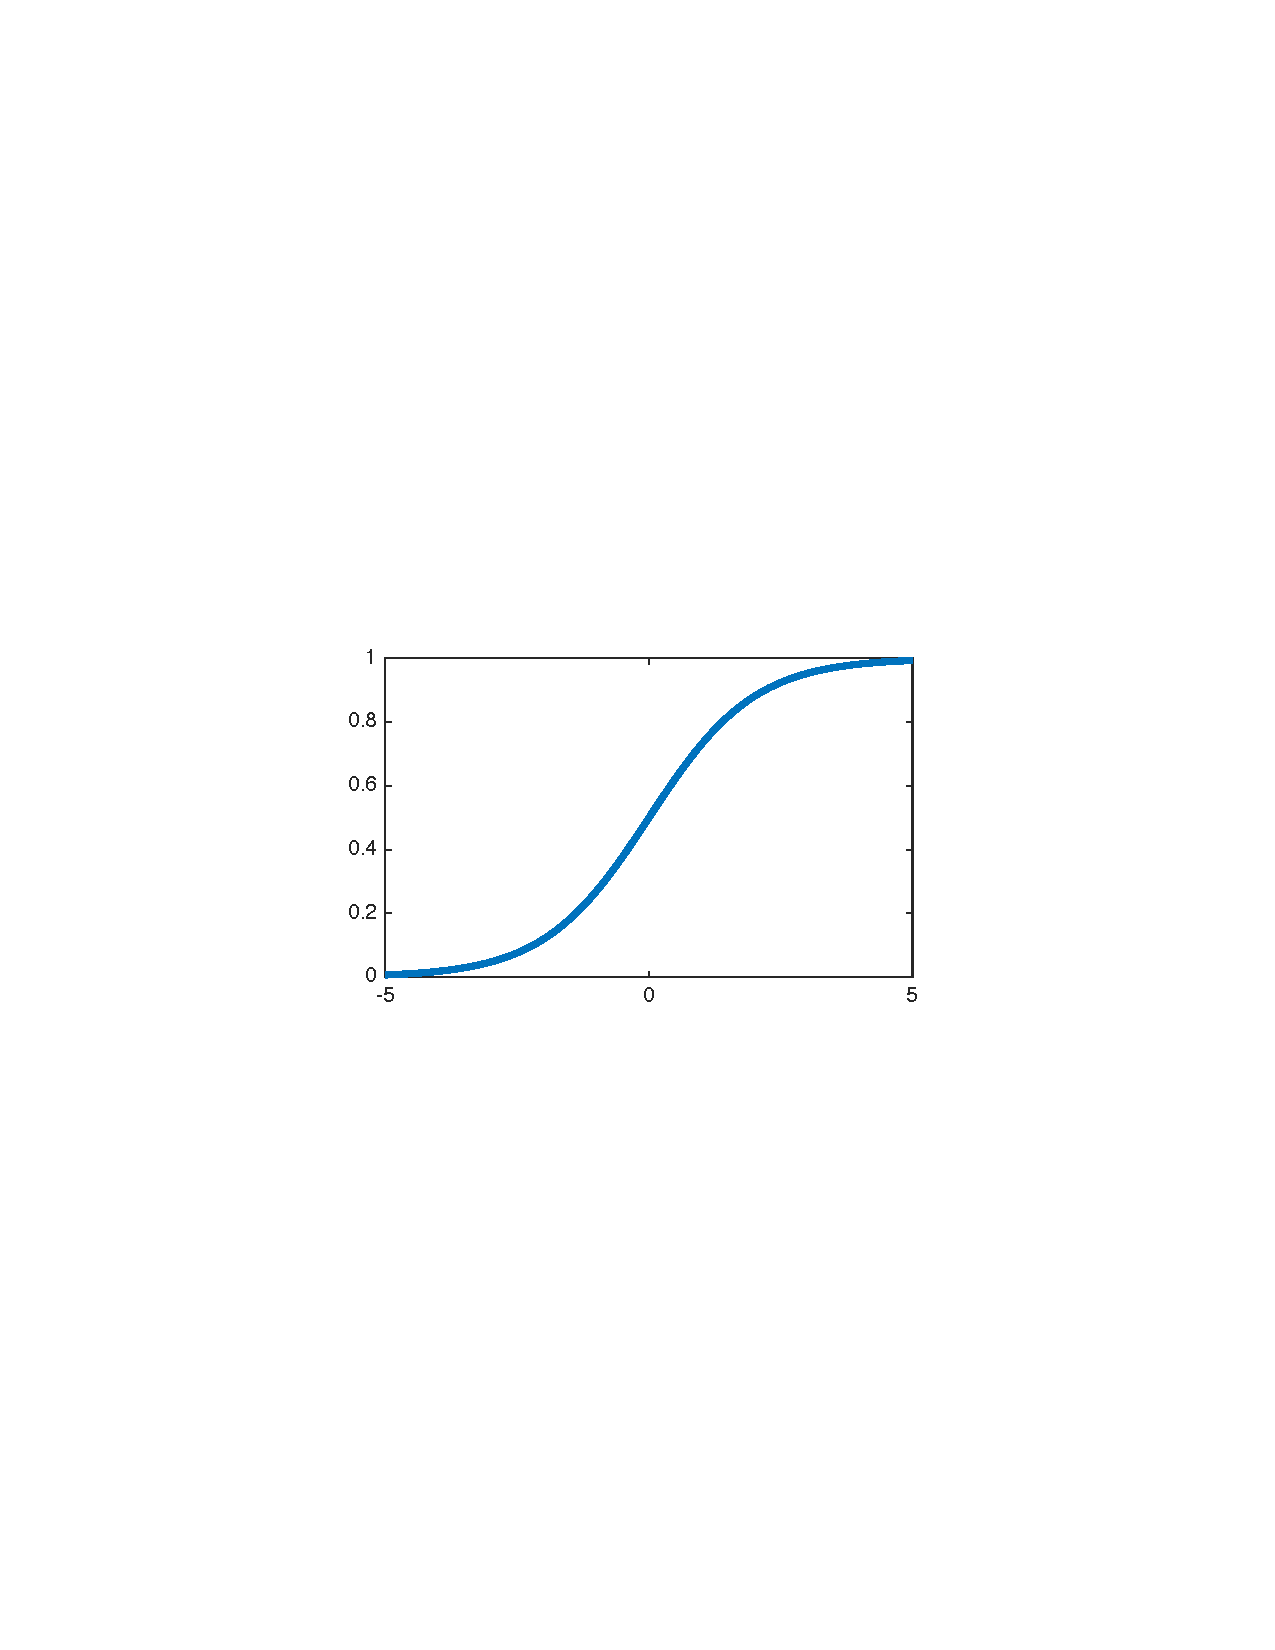
\includegraphics[width=10cm]{images/sigmoidal.pdf}
    \caption{Sigmoidalna (logistička) funkcija}
    \label{fig:sigmoidal}
\end{figure}

Za potrebe ovog rada prilikom učenja neuronske mreže korišten je algoritam propagacije pogreške unatrag te navedena sigmoidalna (logistička) prijenosna funkcija. Navedeni algoritam učenja bit će pobliže opisan u poglavlju o učenju neuronske mreže, no prije toga slijedi kratak osvrt na osnovni model neuronske mreže.

\section{Osnovni model neuronske mreže}

Skup jednostavnih procesnih jedinica, odnosno umjetnih neurona, koji su povezani u paralelne strukture različitih arhitektura naziva se umjetna neuronska mreža. Primjer jedne takve umjetne neuronske mreže prikazan je na slici \ref{fig:neural_net}.
\begin{figure}[htb]
    \centering
    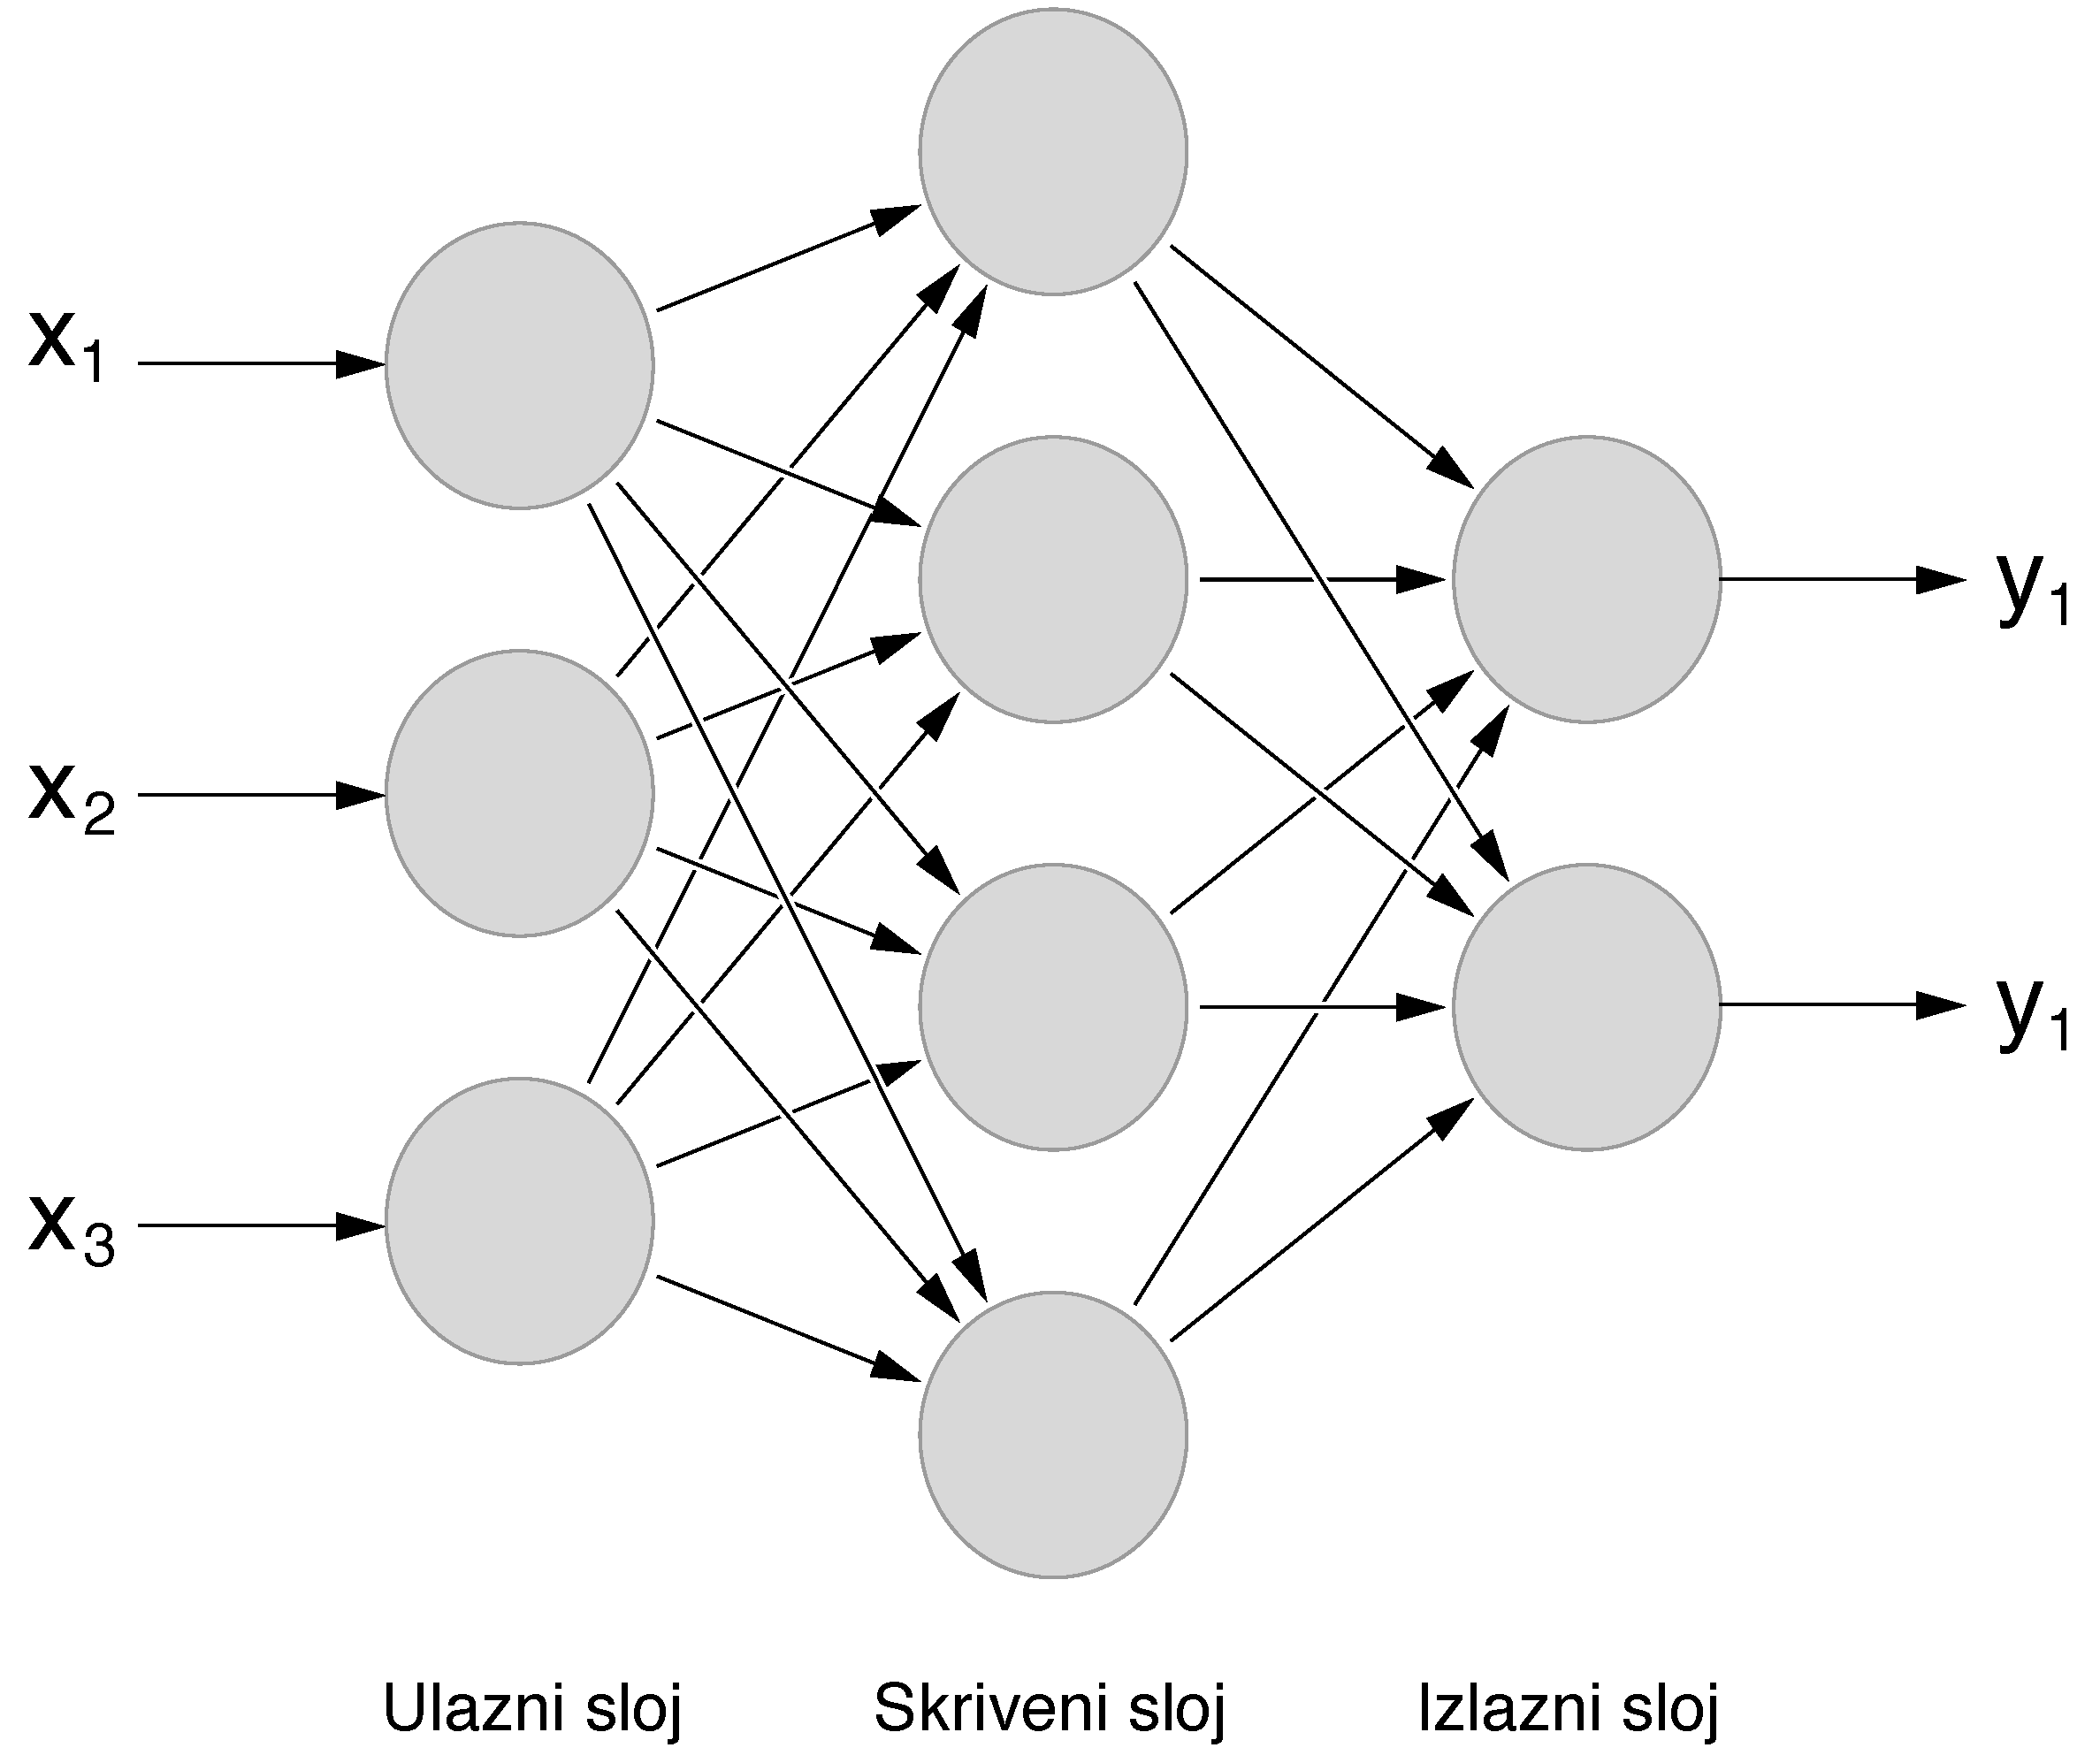
\includegraphics[width=12cm]{images/neural_net.pdf}
    \caption{Primjer potpuno povezane unaprijedne neuronske mreže}
    \label{fig:neural_net}
\end{figure}

S lijeve strane neuronske mreže nalaze se ulazni neuroni. Na njih se dovodi informacija koju je potrebno obraditi te kao takvi ne obavljaju nikakvu obradu već služe samo za prosljeđivanje ulaznih podataka na iduće slojeve mreže. Idući sloj je skriveni sloj, na slici je prikazan samo jedan no unutrašnjost mreže može biti sastavljena od više skrivenih slojeva. Unutar skrivenih slojeva se zbiva obrada informacija. Zadnji sloj, na slici krajnje desni, je izlazni sloj koji nakon obrade podataka dostavlja konačne rezultate okolini.

Arhitektura mreže određena je s više parametara. Jedan od njih je i broj skrivenih slojeva te broj neurona u pojedinom sloju. Mreža prikazana na slici \ref{fig:neural_net} je strukture \mbox{$3 \times 4 \times 2$} (pojedini sloj je odvojen znakom $\times$, te brojka predstavlja broj neurona u pojedinom sloju). Također, povezanost među neuronima određuje arhitekturu mreže. Mreža iz primjera je potpuno povezana slojevita, jer su neuroni iz sloja $n$ povezani sa svim neuronima iz sloja $n+1$, gledano s lijeva na desno. Prikazana mreža je među ostalim i unaprijedna mreža jer je smjer poveznica pojedinog sloja u smjeru s lijeva na desno, to jest iz smjera $n$ prema $n+1$. Mreža može biti i ciklička, gdje su primjerice neuroni pojedinog sloja povezani u oba pravca.

Za potrebe ovog rada korištena je potpuno povezana unaprijedna slojevita neuronska mreža u ponešto drugačijem broju neurona i skrivenih slojeva. U literaturi se takva mreža često navodi pod imenom višeslojni perceptron \engl{multilayer perceptron}.

\section{Učenje neuronske mreže}

Rad s umjetnim neuronskim mrežama se može podijeliti u dvije faze: prvu fazu ili fazu učenja \engl{training, learning} te drugu fazu ili fazu iskorištavanja kad se naučena neuronska mreža koristi za obradu podataka.

Prilikom faze učenja neuronskoj mreži se na ulaze dovode uzorci iz skupa uzoraka za učenje i kako je već ranije spomenuto da mijenjanje jakosti veza predstavlja učenje tako se i neuronskoj mreži mijenjaju jakosti veza, to jest težine, između međusobno povezanih neurona. Težine se mogu podešavati prilikom predočavanja svakog uzorka što se naziva pojedinačno učenje \engl{on-line learning} ili tek nakon što se mreži predoče svi uzorci iz skupa uzoraka što se naziva grupno učenje \engl{batch learning}. Predočavanje jednog uzorka neuronskoj mreži se naziva \emph{iteracija}, a predočavanje čitavog skupa uzoraka za učenje \emph{epoha}.

Postoji još jedna podjela načina učenja kod neuronskih mreža. Postoji nadzirano učenje \engl{supervised learning} ili učenje s učiteljem gdje se mreži predočavaju uzorci oblika $f(ulaz, zeljeni\ izlaz)$, a zadaća je mreže naučiti ispravno klasificirati pojedini uzorak. Kod učenja bez učitelja \engl{unsupervised learning}, uzorci koje dobiva neuronska mreža su oblika $\{(ulaz), ...,(ulaz)\}$ te mreža tada obavlja grupiranje podataka u pojedine razrede. Postoji još i podržano učenje \engl{reinforcement learning} gdje se mreža koristi kao model za aproksimaciju Q-vrijednosti stanja i akcija.

Prilikom učenja neuronske mreže cilj je postići da mreža dobro generalizira podatke iz domene koji su predočeni skupom za učenje. No skup za učenje, to jest bilo koji skup ulaznih podataka, sadrži određenu količinu šuma. Ukoliko se mreža krene prilagođavati prisutnom šumu u skupu podataka za učenje dolazi do pretreniranosti mreže i samim time gubi sposobnost generalizacije. Stoga, od iznimne je važnosti pratiti učenje mreže i onog trenutka kad se počne prilagođavati prisutnom šumu u podacima, to jest počne gubiti sposobnost generalizacije, zaustaviti učenje mreže.

Iz tog razloga, dostupni skup podataka se dijeli na tri podskupa: skup za učenje \engl{training set}, skup za provjeru \engl{validation set} te skup za testiranje \engl{testing set}. Mreža se uči predočavanjem podataka iz skupa za učenje. Učenje takve mreže se povremeno provjerava skupom za provjeru, primjerice nakon svake epohe. Bitno je napomenuti da prilikom te provjere mreži nije dopušteno da se prilagođava podacima iz skupa za provjeru. U početku učenja mreže ukupna greška kod prepoznavanja skupa za učenje i skupa za provjeru će padati, kako je i prikazano na slici \ref{fig:learning_curve}. No u jednom trenutku će se mreža početi prilagođavati šumu u skupu podatak za učenje i u tom trenutku ukupna greška nad skupom za provjeru početi rasti dok će nad skupom za učenje greška nastaviti padati, i zapravo u tom je trenutku potrebno zaustaviti učenje.
\begin{figure}[htb]
    \centering
    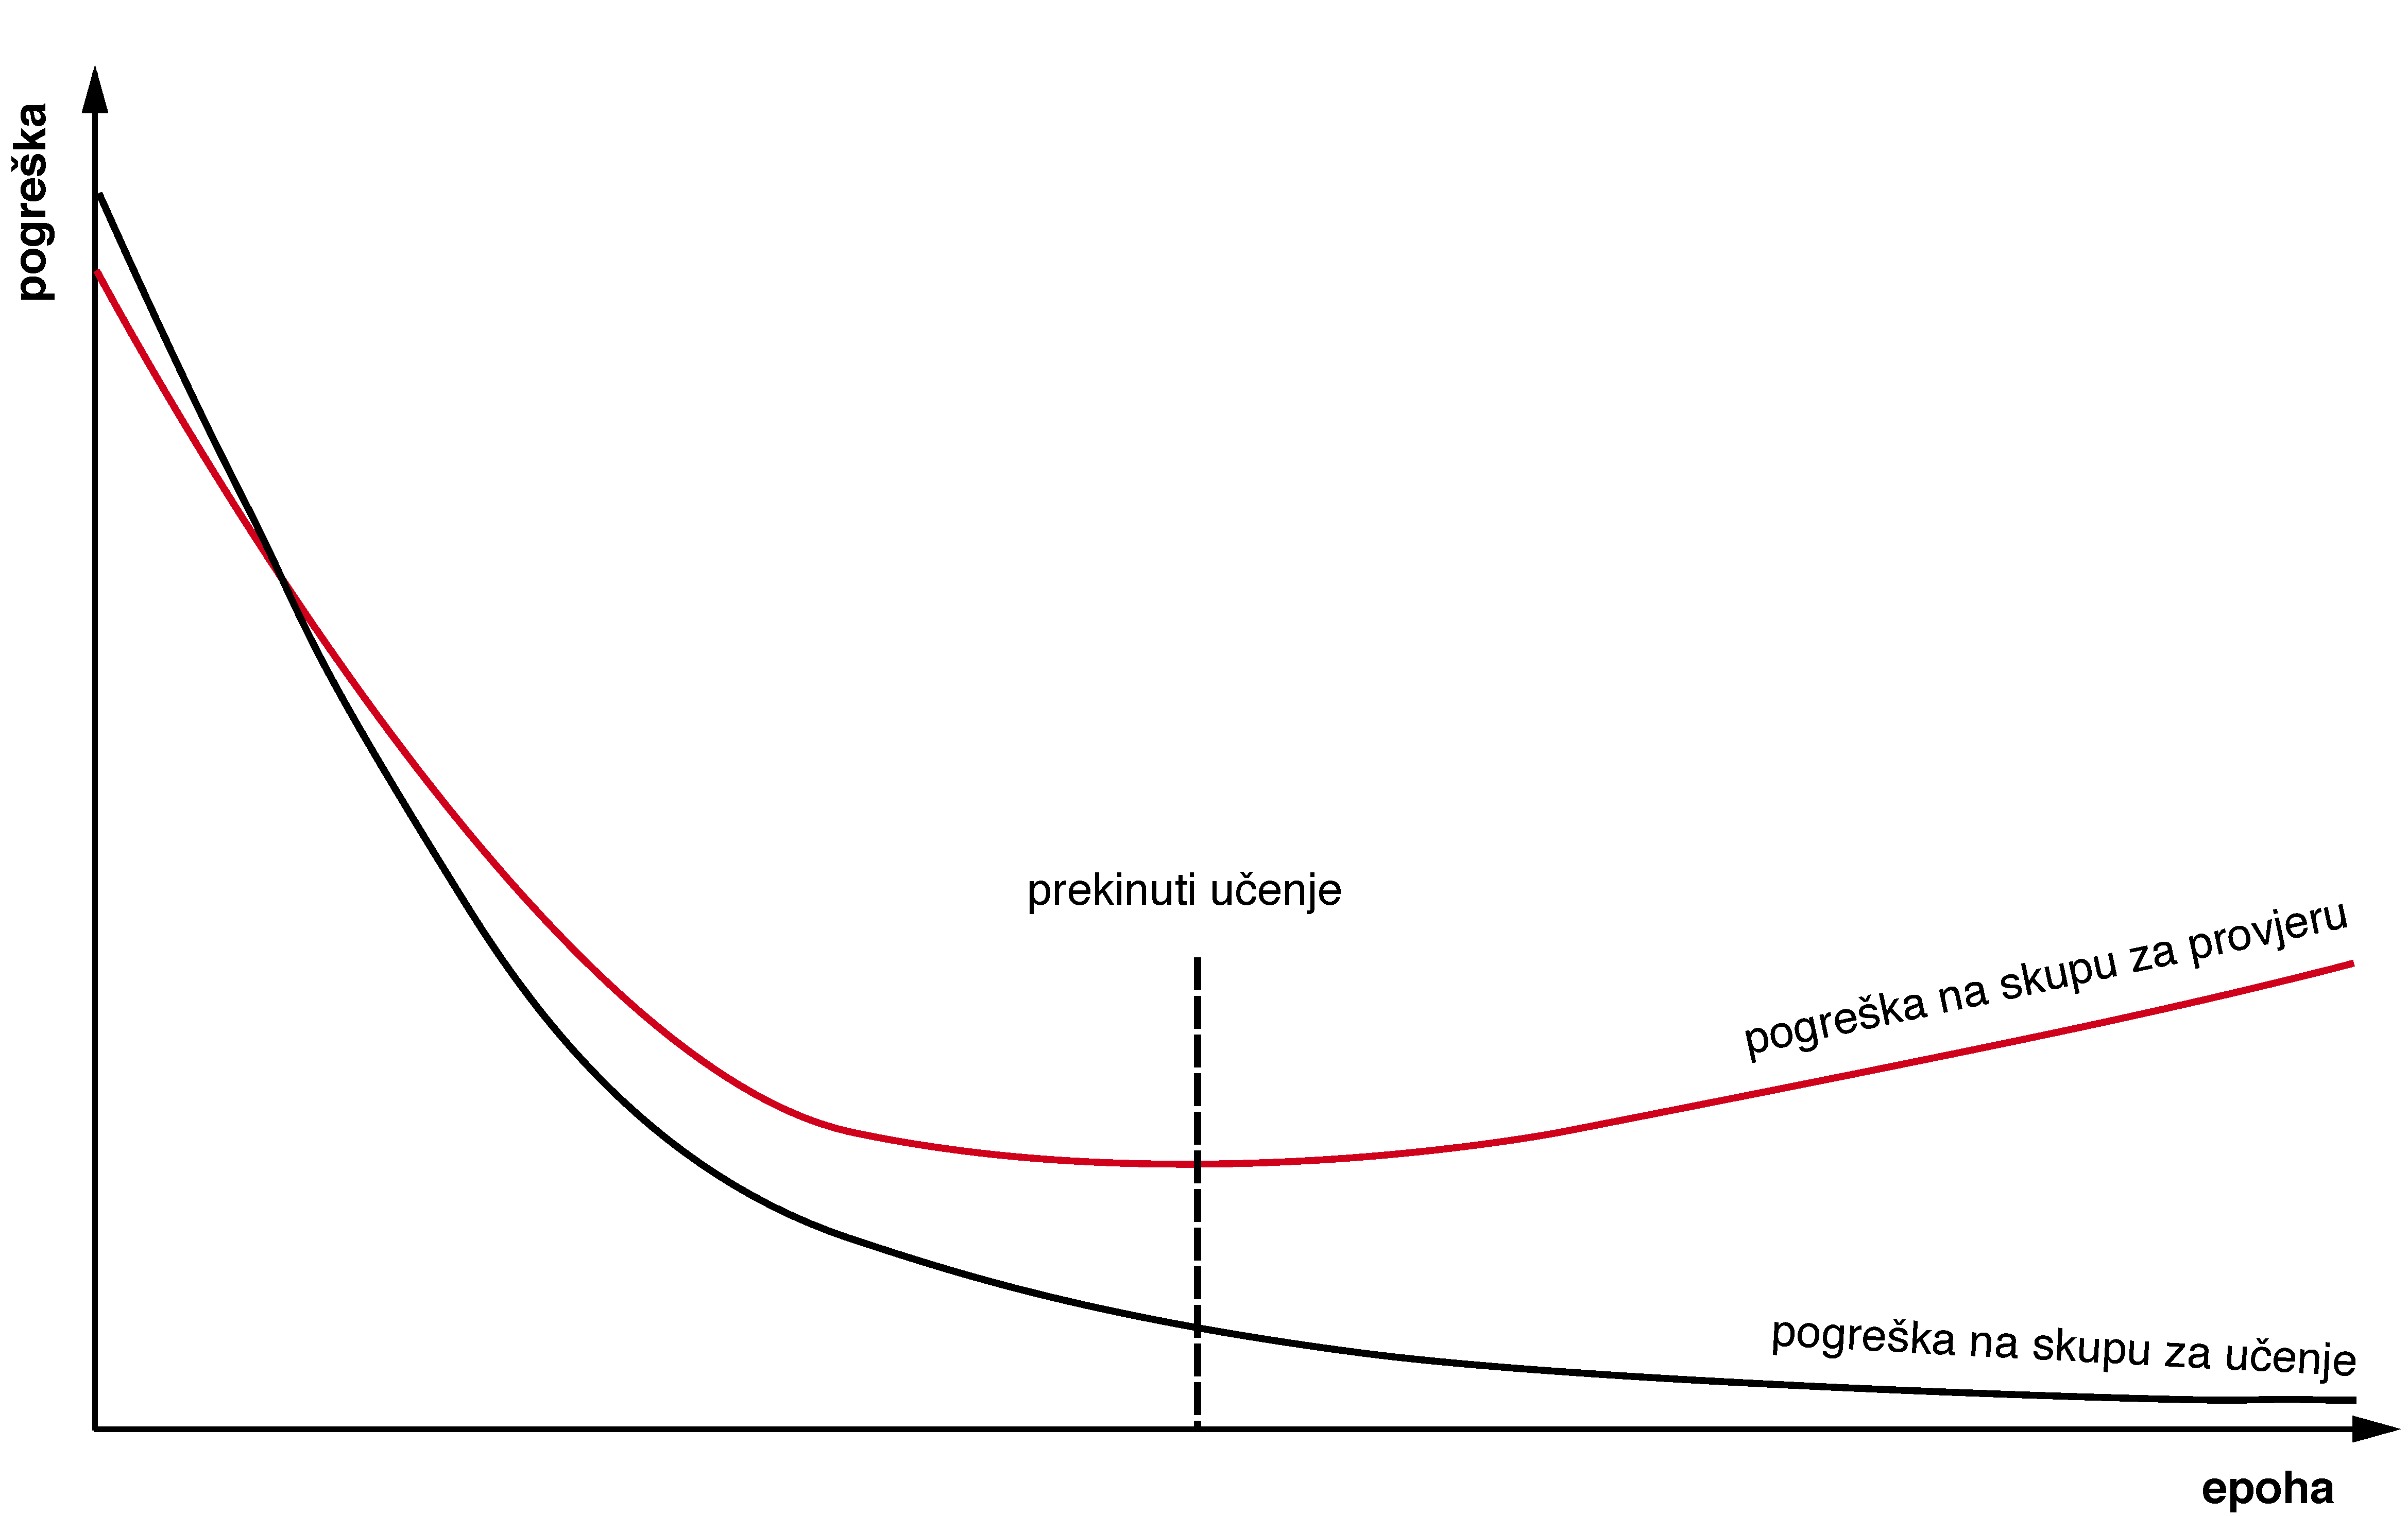
\includegraphics[width=14cm]{images/learning_curve.pdf}
    \caption{Pogreška prilikom učenja neuronske mreže}
    \label{fig:learning_curve}
\end{figure}

Nakon što je učenje završilo, mreža se još jednom provjera nad skupom za testiranje te se time mjeri konačna kvaliteta mreže. Za potrebe ovog rada skup za učenje sadrži 80 \% uzoraka, dok skupovi za provjeru i testiranje sadrže svaki po 10 \% uzoraka.

\section{Učenje algoritmom propagacije pogreške unatrag}

Za potpuno povezanu unaprijednu višeslojnu neuronsku mrežu koja koristi sigmoidalnu (logističku) prijenosnu funkciju kao metoda učenja često se odabire algoritam propagacije pogreške unatrag. Upravo takva vrsta mreže i prijenosne funkcije je korištena za potrebe ovog rada, te će i objašnjenje algoritma pratiti navedena svojstva.

Pojedini uzorak iz skupa za učenje specificiran je ulazom i željenim izlazom koji mreža mora naučiti. Za mrežu koja ima $n$ ulaza te $m$ izlaza, skup za učenje koji se sastoji od $N$ uzoraka će biti oblika $\{(x_{1,1}, ..., x_{1,n}) \rightarrow (t_{1,1}, ..., t_{1,m}), ..., (x_{N,1}, ..., x_{N,n}) \rightarrow (t_{N,1}, ..., t_{N,m})\}$. Predočavanjem pojedinog uzorka mreža će na svom izlaznom sloju davati podatke u skladu s naučenim težinama. Za $i$-ti uzorak iz skupa za učenje mreža će izgenerirati izlaz u obliku $(o_{i,1}, ..., o_{i,m})$. Odstupanje između očekivanoga i dobivenoga izlaza predstavlja grešku za pojedini uzorak, stoga će se ukupna pogreška za $k$-ti uzorak računati kao ukupno kvadratno odstupanje, to jest računati će se kao suma po svakom izlaznom neuronu od kvadrata razlike željene vrijednosti i dobivene vrijednosti, te sve podijeljeno s dva:
\begin{equation}
    E(k) = \frac{1}{2}\sum_{i=1}^{m} (t_{k,i}-o_{k,i})^2.
\end{equation}

Ukupna prosječna pogreška koju neuronska mreža radi nad čitavim skupom za učenje koji se sastoji od $N$ uzoraka definirana je izrazom:
\begin{equation}
    E = \frac{1}{N}\sum_{k=1}^{N} E(k).
\end{equation}

Algoritam propagacije pogreške unatrag dobiva se primjenom algoritma gradijentnog spusta na problem minimizacije funkcije pogreške. Korak algoritma propagacije pogreške unatrag se ponavlja sve dok nije zadovoljen uvjet zaustavljanja, što može biti maksimalni broj iteracija, minimalna pogreška ili već navedeni postupak kada se rezultat učenja provjerava skupom za provjeru nakon svake epohe ili nakon nekoliko njih.

Prije početka učenja neuronske mreže, težine se postavljaju na slučajne vrijednosti. Zatim, sljedeći koraci se ponavljaju sve dok nije zadovoljen uvjet zaustavljanja. Za svaki uzorak $s : (x_{s,1}, ..., x_{s,n}) \rightarrow (t_{s,1}, ..., t_{s,m})$ iz skupa za učenje se čini sljedeće:
\begin{enumerate}
  \item Podaci $(x_{s,1}, ..., x_{s,n})$ se postavljaju na ulaz mreže.
  \item Izračunaju se izlazi svih neurona, gdje su izlazni neuroni mreže označeni s $(o_{s,1}, ..., o_{s,m})$.
  \item Odredi se pogreška svakog od neurona izlaznog sloja, gdje je pogreška $i$-tog izlaznog neurona označena s $\delta_i ^ K$ te definirana izrazom:$$\delta_i ^ K = o_{s,i}\cdot (1-o_{s,i})\cdot(t_{s,i}-o_{s,i}).$$Bitno je napomenuti da je dani izraz definiran nad neuronskom mrežom koja koristi sigmoidalnu (logističku) prijenosnu funkciju te izraz $o_{s,i}\cdot(1-o_{s,i})$ predstavlja njezinu derivaciju.
  \item Zatim se odrede pogreške neurona u svim skrivenim slojevima gdje se pogreška neurona računa kao težinska suma pogrešaka neurona kojima trenutni neuron šalje svoj izlaz, pomnoženu derivacijom prijenosne funkcije tog neurona:$$\delta_i^{(k)} = y_i^{(k)}\cdot(1-y_i^{(k)})\cdot\sum_{d \in Downstream} w_{i,d}\cdot\delta_d^{(k+1)}.$$
  \item Napraviti korekciju svih težina kako je opisano izrazom:$$w_{i,j}^{(k)} \leftarrow w_{i,j}^{(k)} + \eta\cdot y_i ^ {(k)}\cdot\delta_j^{(k+1)},$$ gdje $\eta$ predstavlja stopu učenja \engl{learning rate}.
\end{enumerate}

 Stopa učenja je obično dosta malen broj, u intervalu između $0$ i $1$. Za velike vrijednosti stope učenja algoritam će vrlo vjerojatno divergirati te naučena mreža neće biti naučena. Također, ukoliko je stopa učenja premalena algoritam će vrlo vjerojatno konvergirati ka lokalnom minimumu te naučena mreža neće imati najbolja moguća svojstva. Dakle, brzina kojim se stiže do minimuma ovisi o stopi učenja.
 
 Kako bi se izbjegao problem konvergiranja algoritma ka lokalnom minimumu, navedeni izraz za korekciju težina se modificira imajući u vidu jednu analogiju iz stvarnog svijeta: moment inercije \citep{umjnm}. Ukoliko se položaj na plohi pogreške zamisli kao položaj loptice, i ako ta loptica nema inercije tada će se ta loptica spustiti u prvi lokalni minimum i tamo ostati, kako je i prikazano na slici \ref{fig:momentum}.
 \begin{figure}[htb]
    \centering
    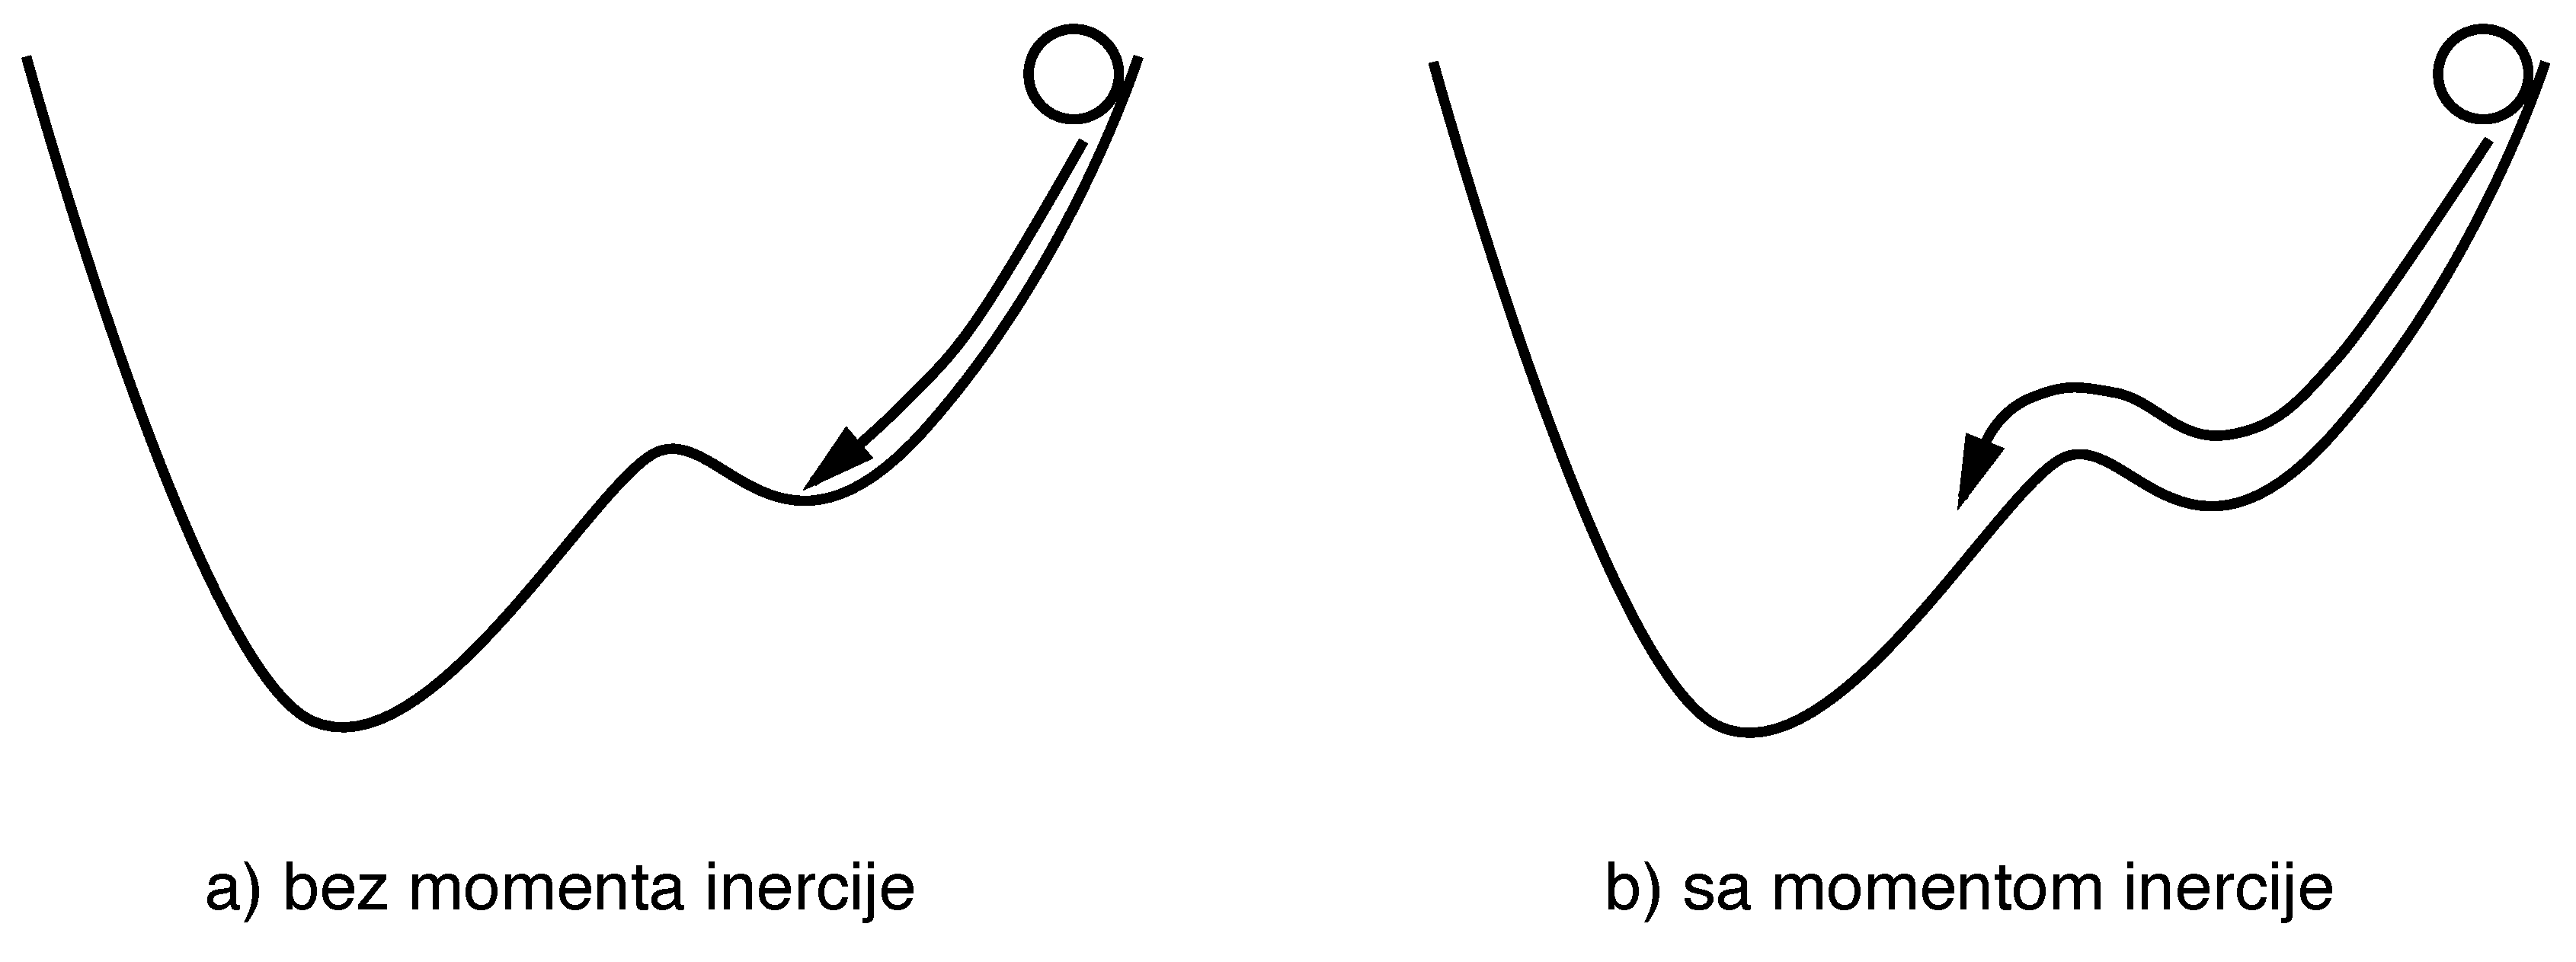
\includegraphics[width=14cm]{images/momentum.pdf}
    \caption{Učenje uz moment inercije}
    \label{fig:momentum}
\end{figure}

No ukoliko loptica ima moment inercije, ona će se nastaviti gibati te ako je lokalni minimum dovoljno malen, loptica će ga napustiti i nastaviti gibanje prema globalnom minimumu. Izraz za korekciju težina pri kojoj se koristi moment inercije je:$$w_{i,j}^{(k)} \leftarrow w_{i,j}^{(k)} + \eta\cdot y_i ^ {(k)}\cdot \delta_j^{(k+1)} + \alpha\cdot\Delta w_{i,j}^{(k)'},$$ gdje $\alpha$ predstavlja moment inercije, što je obično u intervalu od $0$ do $1$, te $\Delta w_{i,j}^{(k)'}$ predstavlja vrijednost korekcije iz prethodnog koraka.
